\section{Лекция 15 (09.11)}

\subsection{Аппроксимация уравнения переноса с ограничением потока}

\subsubsection{Схемы первого и второго порядка точности}
Рассмотрим уравнение переноса в одномерной постановке

\begin{equation*}
\label{eq:tvd_transport}
\dfr{u}{t} + U\dfr{u}{x} = 0
\end{equation*}
Все дальнейшие выкладки будем приводить исходя из условия положительности скорости переноса $U > 0$.

Рассмотрим два вида пространственной аппроксимации конвективного слагаемого на равномерной сетке: схемой против потока и симметричной схемой
\begin{align}
& \dfr{u_i}{t} + U \frac{u_i - u_{i-1}}{h} = 0, \label{eq:tvd_upwind}\\
& \dfr{u_i}{t} + U \frac{u_{i+1} - u_{i-1}}{2h} = 0. \label{eq:tvd_sym}
\end{align}
Первая схема является (условно) устойчивой но при этом обладает первым
порядком аппроксимации. Вторая неустойчива, но имеет порядок $o(h^2)$.
Идея методов аппроксимации с ограничением потока состоит в том,
чтобы на основе комбинации первой и второй схем
построить устойчивое решение, имеющее ``почти везде'' второй порядок аппроксимации.

Запишем эти аппроксимации в общем виде:
\begin{equation}
\label{eq:tvd_appr_with_f}
\dfr{u_i}{t} = \frac{f_{i-\sfrac12} - f_{i+\sfrac12}}{h}.
\end{equation}
Здесь $f_{i+\sfrac12}$ -- численный поток, который в зависимости от выбранной схемы будет равен
\begin{equation}
\label{eq:tvd_fhl}
\begin{aligned}
&f^L_{i+\sfrac12} = U u_i                            &\text{-- схема против потока}\\
&f^H_{i+\sfrac12} = U \frac{u_i + u_{i+1}}{2}        &\text{-- симметричная схема}.
\end{aligned}
\end{equation}
Здесь $f^L$, $f^H$ означают потоки низкого (Low) и высокого (High) порядка аппроксимации.

Аппроксимацию с ограничением потока запишем в виде
\begin{equation}
\label{eq:tvd_f}
f_{i+\sfrac12} = f^L_{i+\sfrac12} + \Phi_{i+\sfrac12} \left( f^H_{i+\sfrac12} - f^L_{i+\sfrac12} \right).
\end{equation}
$\Phi$ в этой записи называется ограничителем, который служит
переключателем: при $\Phi = 0$ мы получаем схему первого порядка, при $\Phi=1$ -- схему второго порядка.

Далее будем выбирать $\Phi$ таким образом, чтобы не допустить возникновения осцилляций в численном решении.

\subsubsection{Условие TVD}
В качестве критерия, характеризующего возникновение и развитие осцилляций, выберем полную вариацию:
\begin{equation}
\label{eq:tvd_tv}
\begin{WithArrows}
TV(u) =& \displaystyle\int\left| \nabla u \right|\,dx =           \Arrow{в одномерном случае}\\[10pt]
      =& \displaystyle\int\left| \dfr{u}{x} \right| \, dx =       \Arrow{для сеточной функции}\\[10pt]
      =& \displaystyle\sum_{i}\left| u_i - u_{i-1}\right|.
\end{WithArrows}
\end{equation}
Условие уменьшения осцилляций в решении на следующем временном слое примет вид
\begin{equation*}
TV(\hat u) \leq TV(u).
\end{equation*}
Численные схемы, удовлетворяющие этому условию, называются TVD (Total variation diminishing) схемами.

Запишем численную схему в общем виде
\begin{equation}
\label{eq:tvd_harten}
\dfr{u_i}{t} = c_{i-\sfrac12} (u_{i-1} - u_{i}) + c_{i+\sfrac12} (u_{i+1} - u_{i}).
\end{equation}
Согласно теореме Хартена такая схема удовлетворяет свойству TVD, если $c_{i\pm\sfrac12} \geq 0$.
Схема против потока \cref{eq:tvd_upwind} является TVD-схемой:
$$c_{i-\sfrac12} = \frac{U}{h}, \quad c_{i+\sfrac12} = 0,$$
а симметричная схема \cref{eq:tvd_sym} -- нет:
$$c_{i-\sfrac12} = \frac{U}{2h}, \quad c_{i+\sfrac12} = -\frac{U}{2h}.$$

Подставляя уравнение \cref{eq:tvd_f} в \cref{eq:tvd_appr_with_f} 
и приводя к форме \cref{eq:tvd_harten} получим
\begin{equation}
\label{eq:tvd_phi_condition1}
\dfr{u_i}{t} = \frac{U}{2h}\left( 2 - \Phi_{i-\sfrac12} \right) \left( u_{i-1} - u_{i} \right)
               +\frac{U}{2h}\left(-\Phi_{i+\sfrac12} \right) \left( u_{i+1} - u_i\right)
\end{equation}
То есть для удовлетворения свойства TVD необходимо, чтобы $\Phi \leq 0$.
Для второго порядка точности требуется $\Phi = 1$. То есть линейные схемы TVD не могут иметь высокий порядок точности.

\subsubsection{Нелинейные TVD схемы}
Для того, чтобы преодолеть это ограничение, будем строить нелинейные схемы.
Общая идея построения таких схем состоит в том, чтобы выбрать такую $\Phi$,
при которой второе слагаемое равенства \cref{eq:tvd_phi_condition1} можно
было отнести к первому. То есть можно бы было записать
\begin{equation}
\label{eq:tvd_phi_condition2}
\Phi_{i+\sfrac12}(u_{i+1} - u_{i}) = -\Phi'_{i+\sfrac12} (u_{i-1} - u_{i}).
\end{equation}
Тогда условием TVD станет выражение
\begin{equation}
\label{eq:tvd_phi_condition3}
2 - \Phi_{i-\sfrac12} + \Phi'_{i+\sfrac12} \geq 0.
\end{equation}

Для характеристики поведения функции выберем соотношение наклонов (slope ratio),
который в одномерном виде запишется в виде:
\begin{equation}
\label{eq:tvd_ri}
r_i = \frac{u_i - u_{i-1}}{u_{i+1} - u_{i}}
\end{equation}
Нелинейность схемы будет выражаться в зависимости
\begin{equation*}
\Phi_{i+\sfrac12} = \Phi(r_i).
\end{equation*}

Из \cref{eq:tvd_phi_condition2} следует
\begin{equation*}
\Phi'_{i+\sfrac12} = \frac{\Phi(r_i)}{r_i}
\end{equation*}
а неравенство $\label{eq:tvd_phi_condition4}$
перепишется в виде
\begin{equation*}
\label{eq:tvd_phi_condition5}
2 - \Phi(r_i) + \frac{\Phi(r_i)}{r_i} \geq 0.
\end{equation*}
Чтобы из этого условия получить ограничение для $\Phi$, явно не зависящее от $r_i$, потребуем
\begin{equation}
\label{eq:tvd_phi_condition4}
\Phi\left(\frac{1}{r_i}\right) = \frac{\Phi(r_i)}{r_i}.
\end{equation}
Тогда неравентсво \cref{eq:tvd_phi_condition3} примет вид
\begin{equation*}
\label{eq:tvd_phi_condition6}
2 - \Phi(r_i) + \Phi\left(\frac{1}{r_i}\right) \geq 0.
\end{equation*}
Отсюда получим условие для $\Phi$:
\begin{equation}
\label{eq:tvd_phi_condition7}
0 \leq \Phi(r_i) \leq 2.
\end{equation}

Дополнительно потребуем, чтобы в точках с гладким поведением функции использовать схему второго порядка точности:
\begin{equation}
\label{eq:tvd_phi_condition8}
\Phi(1) = 1
\end{equation}
а в точках локального экстремума (которые особенно подвержены появлению осцилляций) гарантировать переключение на схему первого порядка:
\begin{equation}
\label{eq:tvd_phi_condition9}
\Phi(r\leq0) = 0.
\end{equation}

Таким образом, для построения TVD схемы, функция ограничитель должна удовлетворять условиям
\cref{eq:tvd_phi_condition4,eq:tvd_phi_condition7,eq:tvd_phi_condition8,eq:tvd_phi_condition9}.
Ниже представлены некоторые часто используемые ограничители, удовлетворяющие этим свойствам:
\begin{equation}
\label{eq:tvd_limiter}
\Phi(r) = \left\{
\begin{array}{ll}
\max(0, \min(r, 1))                   & \text{-- minmod};\\[10pt]
\dfrac{r + |r|}{1+|r|}                & \text{-- Van Leer}; \\[10pt]
\max(0, \min(2r, \dfrac{1+r}{2}, 2)   & \text{-- monotonized central (MC)}; \\[10pt]
\max(0, \min(2, r), \min(1, 2 r))     & \text{-- superbee}.
\end{array}
\right.
\end{equation}

\subsection{TVD-схемы для неструктурированных конечнообъёмных сеток}
Рассмотрим многомерное уравнение переноса
\begin{equation}
\nonumber
\dfr{u}{t} + \vec U \cdot \nabla u = 0.
\end{equation}

Применим конечнообъёмную процедуру
для получения слабой интегральной постановки задачи.
Для этого проинтегрируем это уравнение
по конечному объёму $E_i$ 
и применим формулу интегрирования по частям.
Получим
\begin{equation}
\label{eq:tvd_fvm_transport}
\left| V_i \right|
\dfr{u}{t}
+ \sum_{j\in {\rm nei}(i)} {f_{ij} \left|\gamma_{ij}\right|}
= 0, \quad f_{ij} = u_{ij} U_{ij}.
\end{equation}
Здесь $|V_i|$ -- объём конечного элемента,
${\rm nei}(i)$ -- совокупность
всех точек коллокации, инцидентных ячейке $i$
(центров соседних ячеек и соседних граничных граней),
$f_{ij}$ -- поток из точки коллокации $i$ в точку коллокации $j$,
$|\gamma_{ij}|$ --
площадь грани
конечного объёма $i$, через
которую этот объём соединяется с точкой коллокации $j$,
$u_{ij}$ -- значение функции $u$, отнесённое к этой грани,
$U_{ij}$ -- скорость потока в направлении внешней по отношению
к ячейке $i$ нормали.

Для потока справедливо
\begin{equation}
\label{eq:tvd_fij_fji}
f_{ij} = -f_{ji}.
\end{equation}
То есть для вычисления потока на грани достаточно найти значение для одного направления.
Выберем это направление $\overrightarrow{ij}$ таким образом, чтобы $U_{ij} > 0$ (рис.~\ref{fig:fvm_tvd}).


\begin{figure}[h!]
\centering
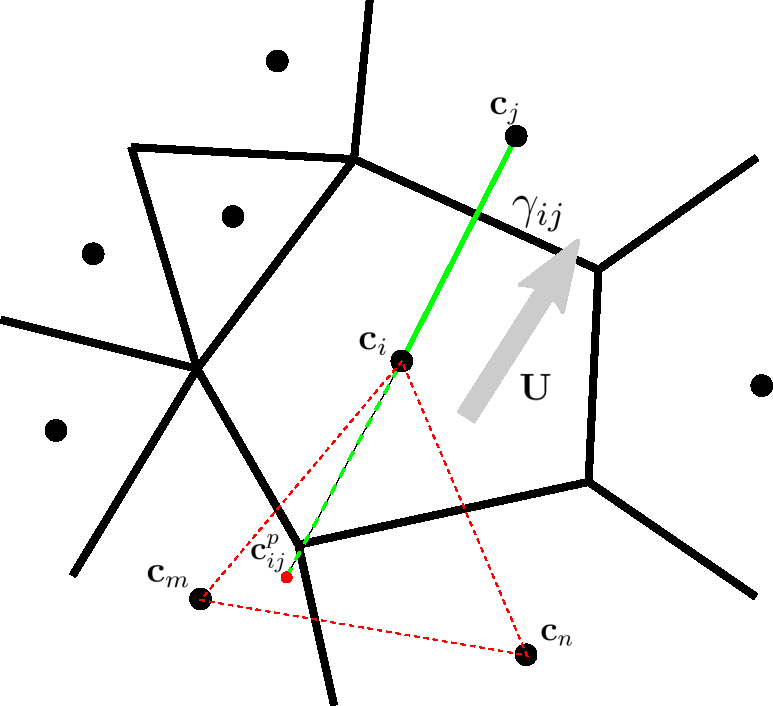
\includegraphics[width=0.4\linewidth]{fvm_tvd.pdf}
\caption{Вспомогательный узел $\vec c^p_{ij}$ на конечнообъёмной сетке}
\label{fig:fvm_tvd}
\end{figure}

Будем считать, что скорость переноса $U$ -- известная функция.
Тогда запишем значения потоков высокого и низкого порядка согласно \cref{eq:tvd_fhl}:
\begin{equation}
\label{eq:tvd_fhl_fvm}
\begin{aligned}
&f^L_{ij} = U_{ij} u_i                 &\text{-- схема против потока}\\
&f^H_{ij} = U_{ij} \frac{u_i + u_j}{2} &\text{-- симметричная схема}.
\end{aligned}
\end{equation}

Поток при этом запишется по аналогии с \cref{eq:tvd_f}:
\begin{equation}
\label{eq:tvd_f_fvm}
f_{ij} = f^L_{ij} + \Phi(r_{ij}) \left( f^H_{ij} - f^L_{ij} \right).
\end{equation}

В одномерном случае для записи соотношения наклонов $r_i$ \cref{eq:tvd_ri} использовались
три точки: текущий узел $i$, узел против потока $i-1$, и узел по потоку $i+1$.
Для случае неструктурированной сетки лишь две из этих трёх точек являются
узлами коллокации: текущий узел $i$ и узел по потоку $j$. Определим точку
против потока симметричным отражением: $\vec{c}^p_{ij} = 2\vec c_i - \vec c_j$ (см. рис.~\ref{fig:fvm_tvd}).
Значение функции в этой точке обозначим как $u^p_{ij}$.
Тогда соотношение наклонов запишется в виде

\begin{equation}
\label{eq:tvd_ri_fvm}
r_i = \frac{u_i - u_{ij}^p}{u_j - u_i}
\end{equation}

Точка $\vec c^p$ (в отличии от $x_{i-1}$ из одномерного случая)
не является точкой коллокации. То есть
значение $u^p$ нельзя достать из вектора столбца сеточной функции $u$.
Однако, это значение можно интерполировать
по значениям в ближайших точках коллокации.

\subsubsection{Прямая интерполяция противопоточного значения}
\label{sec:direct_interpolate_up}
Так, в двумерном случае для определения $u^p_{ij}$
необходимо найти три точки коллокации,
ближайшие к точке $\vec c^p_{ij}$ и не лежащие на одной прямой (или две точки коллокации, помимо $c_i$). На рис.~\ref{fig:fvm_tvd}
они помечены индексами $\vec c_m$, $\vec c_n$).
И далее в треуольнике, образованном этими тремя
точками ($\triangle_{imn}$) провести
интерполяцию
по формуле \cref{eq:simplex_interp_2d}.
Специально отметим, что точка $\vec c^p_{ij}$
не обязана содержаться внутри 
треугольника $\triangle_{imn}$.

\subsubsection{Интерполяция противопоточного значения через значение градиентов}
\label{sec:grad_inteprolate_up}.
Другой подход к определению $u^p_{ij}$ основан на записи симметричной конечной разности
по направлению $\vec c_{ij}$:
\begin{equation*}
\left.\dfr{u}{c_{ij}}\right|_i = \frac{u_j - u^p_{ij}}{2|\vec c_{ij}|} \qquad \hence
u_{ij}^p = u_j - 2 |\vec c_{ij}| \left. \dfr{u}{c_{ij}}\right|_i.
\end{equation*}
Производная по направлению $c_{ij}$ находится как проекция градиента:
\begin{equation*}
|\vec c_{ij}| \left.\dfr{u}{c_{ij}}\right|_i = \vec c_{ij} \cdot (\nabla u)_i.
\end{equation*}
Таким образом, задача интерполяции сводится к задаче определения градиента функции
$u$ в узлах коллокации.

\subsubsection{Определение градиентов в узлах коллокации. Метод наименьших квадратов}

Будем рассматривать узел $i$, имеющий $N_i$ соседних узлов $j$.
Для каждого $j$ можно записать линейное приближение
\begin{equation*}
u_j = u_i + |\vec c_{ij}| \dfr{u}{c_{ij}} = u_i + \vec c_{ij} \cdot \nabla u, \qquad j = \overline{0, N_i-1}.
\end{equation*}
Для двумерного случая можно записать:
\begin{equation*}
(\vec c_{ij})_x \, \dfr{u}{x} + (\vec c_{ij})_y \, \dfr{u}{y} = u_j - u_i, \qquad j = \overline{0, N_i - 1}.
\end{equation*}
Это выражение -- есть система линейных уравнений с двумя неизвестными $\dsfr{u}{x}$, $\dsfr{u}{y}$ 
и $N_i$ строками. Запишем её в матричном виде:
\begin{equation*}
\begin{array}{llll}
A y = f, &  \text{ где } & A_{j0} = (\vec c_{ij})_x & \quad A_{j1} = (\vec c_{ij})_y,\\
         &               & y_{0} = \dsfr{u}{x}      & \quad y_{1} = \dsfr{u}{y},\\
         &               & f_{j} = u_j - u_i &.
\end{array}
\end{equation*}
В двумерном случае размерность матрицы $A$ есть $[N_i, 2]$
(для трёхмерной задачи следуя аналогичным рассуждениям получим матрицу с размерностью $[N_i, 3]$).

При этом в двумерном случае у конечного элемента будет минимум три грани (или четыре в трёхмерном случае). То есть $N_i \geq 3$ 
и полученная система имеет неизвестных больше, чем количество уравнений.
Эта система в общем случае не имеет точного решения,
но можно найти такие $y$, при котором невязка будет минимальной.
Определим невязку как 
$$
r_i = \sum_{j=0}^{N_i}\left(A_{ij}y_j\right) - f_i, \qquad i=0, 1.
$$
и будем минимизировать её квадрат
$$
F = \sum_i r_i^2 \to \min
$$
Запишем условие экстремума как
$$
\dfr{F}{y_i} = 2 \sum_j r_j \dfr{r_j}{y_i} =
               2 \sum_j \left( \sum_k \left( A_{jk} y_k\right) - f_j \right)A_{ji} = 0, \qquad i=0,1.
$$
Отсюда получим систему уравнений
$$
\sum_j \left( A_{ji} \sum_k \left( A_{jk} y_k\right) \right) = \sum_j A_{ji}f_j = 0, \qquad i=0,1.
$$
Или, возвращаясь к матричной записи,
$$
A^{T} A y = A^{T}f.
$$
Полученная система имеет размерность $2\times2$ (или $3\times3$ в трёхмерном случае).
Значение компонент градиента в точке коллокации запишется как её прямое решение:
$$
y = \left(A^T A\right)^{-1} A^T f.
$$
Отметим, что матрица $A$ зависит только от геометрии сетки.
Поэтому в программной реализации матричное выражение $\left(A^T A\right)^{-1} A^T $ может быть расчитано 
один раз для каждого узла коллокации на этапе инициализации.
Тогда определение градиента в центрах ячеек на этапе решения задачи 
сведётся к сборке вектора $f$ и умножении его на это выражение.

\subsubsection{Реализация для явной схемы}
Для примера рассмотрим написание TVD-схемы
рассмотрим чисто явную схему для полудискретизованного уравнения \cref{eq:tvd_fvm_transport}:
\begin{equation}
\label{eq:tvd_fvm_explicit_transport}
\left| V_i \right|
\frac{\hat u - u}{\tau}
+ \sum_{j\in {\rm nei}(i)} {f_{ij} \left|\gamma_{ij}\right|}
= 0.
\end{equation}
Для того, чтобы избежать повторного вычисления потоков $f_{ij}$ и $f_{ji}$,
будем собирать эту схему в цикле по граням. Пусть через границу притока нет (то есть для граничные граней $f_{ij} = 0$.
Тогда останется только цикл по внутренним граням:
\begin{equation}
\label{eq:tvd_fvm_assem}
\begin{array}{ll}
\hat u = u                                               & \textrm{-- инициализируем следующий шаг}\\
\textbf{for } s \in\textrm{internal}                     & \textrm{-- цикл по внутренним граням}\\ 
\qquad i,j = \textrm{nei\_cells(s)}                      & \textrm{-- две ячейки, соседние с текущей гранью}\\
\qquad \vec U_{ij}                                       & \textrm{-- вектор скорости в центре грани}\\
\qquad \vec n_{ij}                                       & \textrm{-- вектор нормали к грани от ячейки i к j}\\
\qquad U_{ij} = \vec U_{ij} \cdot \vec n_{ij}            & \textrm{-- проекция скорости на нормаль}\\
\qquad \textbf{if } U_{ij} \leq 0                        & \textrm{-- схема против потока}\\
\qquad \qquad \textrm{swap}(i, j); U_{ij} = -U_{ij}      & \textrm{-- гарантируем, что жидкость течет от $i$ к $j$}\\
\qquad \textbf{endif}                                    & \textrm{}\\
\qquad f^L_{ij} = U_{ij} u_i                             & \textrm{-- поток 1-го порядка \cref{eq:tvd_fhl_fvm}}\\
\qquad f^H_{ij} = U_{ij} (u_i + u_j) / 2                 & \textrm{-- поток 2-го порядка \cref{eq:tvd_fhl_fvm}}\\
\qquad \vec c_i, \vec c_j                                & \textrm{-- центры ячеек}\\
\qquad \vec c^p = 2 \vec c_i - \vec c_j                  & \textrm{-- вспомогательная точка}\\
\qquad u^p = \textrm{interpolate}(i, j, u, \vec c^p)     & \textrm{-- интерполируем $u$ в точке $\vec c^p$}\\
\qquad r = \sfrac{(u_i - u^p)}{(u_j - u_i)}              & \textrm{-- отношение наклонов \cref{eq:tvd_ri_fvm}}\\
\qquad F = \textrm{limiter}(r)                           & \textrm{-- ограничитель \cref{eq:tvd_limiter}}\\
\qquad f_{ij} = f^L_{ij} + F (f^H_{ij} - f^L_{ij})       & \textrm{-- вычисление потока \cref{eq:tvd_f_fvm}}\\
\qquad \hat u_i\minuseq\tau/|V_i|\,f_{ij}\,|\gamma_{ij}| & \textrm{-- добавление в противопотоковую ячейку}\\
\qquad \hat u_j\pluseq \tau/|V_j|\,f_{ij}\,|\gamma_{ij}| & \textrm{-- добавление в попотоковую ячейку}\\
\textbf{endfor}                                          & \\
\end{array}
\end{equation}
Отметим, что использование
противоположенного знака при добавлении в правую
от грани ячейку $j$ связано с тожедством \cref{eq:tvd_fij_fji}.
То есть на самом деле в ячейку $j$
должен бы добавляться поток $f_{ji}$,
но поскольку отдельной обработки этого направления не предусмотрено,
мы добавляем $f_{ij}$ с обратным знаком.
При реализации функции $\textrm{interpolate}$ должен использоваться один из методов, изложенных
в пп.~\ref{sec:direct_interpolate_up}, \ref{sec:grad_inteprolate_up}.

\subsection{Задание для самостоятельной работы}
В тесте \ename{[transport2-fvm-upwind-explicit]}
из файла \ename{transport_fvm_solve_test.cpp}
реализовано решение
двумерного уравнения переноса 
по явной противопотоковой схеме.
Реализация алгоритма
в целом соответствует циклу \cref{eq:tvd_fvm_assem}
с упрощениями, следующими из отсутствия
необходимости вычислять $r$ в схеме против потока (где всегда $F=0$).

Отталкиваясь от этого теста нужно решить двумерное уравнение переноса
с помощью МКО аппроксимации на неструктурированной
сетке.  Использовать постановку из п.~\ref{sec:circle_transport} с $\sigma=0.1$.
Рассмотреть схему против потока и MC TVD-схему пространственной аппроксимации и явную схему для дискретизации по времени.
Для интерполяции противопотокового значения $u^p$ использовать
алгоритм \ref{sec:grad_inteprolate_up}. 

Неструктурированную сетку строить с помощью скрипта \ename{test_data/hexagrid.py}.
Количество элементов сетки подобрать так, чтобы видеть эффект от применения схемы высокого порядка.

\begin{enumerate}
\item
Проиллюстрировать динамику численного решения на неструктурированной конечнообъёмной сетке.
Сравнить решение MC и Upwind.
\item
Для выбранной сетки опытным путём определить максимально допустимый шаг по времени, при котором решение не разваливается;
\item 
Посчитать нормы отклоения полученного численного решения от известного точного (по максимуму и среднеквадратичную):
\begin{align*}
&n_{max} = 1 - \max\limits_{i} (u_i); \\
&n_2 = \left(\dfrac{\sum_i { \left(u_i - u^e(c_i)\right)^2 \left| V_i \right| }}{\sum_i \left| V_i \right|}\right)^{1/2}
\end{align*}
Нарисовать графики этих норм от времени $n(t)$ для двух рассмотренных схем. 
\end{enumerate}

\paragraph{Рекомендации к программированию}
Для вычисления градиентов в центрах ячеек
использовать класс \cvar{FvmCellGradient} из файла \ename{fvm/fvm_assembler.hpp}, экземпляр которого нужно создать на этапе инициализации задачи.
Тогда для вычисления градиентов от известной сеточной функции \cvar{u}
достаточно вызывать метод \cvar{FvmCellGradient::compute}.
